\documentclass[14pt]{beamer}
\usetheme{EastLansing}
\usecolortheme{spruce}

\usepackage{xcolor}
\usepackage{listings}
\usepackage{courier}
\usepackage{graphicx}
\usepackage{amsmath}
\usepackage{algorithm2e}
\usepackage[font=small]{caption}

\usefonttheme[onlymath]{serif}


\definecolor{mGreen}{rgb}{0,0.6,0}
\definecolor{mGray}{rgb}{0.5,0.5,0.5}
\definecolor{mPurple}{rgb}{0.8,0,0.82}
\definecolor{backgroundColour}{rgb}{0.95,0.95,0.92}
\definecolor{lightBlue}{rgb}{0.1, 0.1, 0.8}

\lstdefinestyle{CStyle}{
    backgroundcolor=\color{backgroundColour},   
    commentstyle=\color{mGreen},
    keywordstyle=\color{magenta},
    numberstyle=\tiny\color{mGray},
    stringstyle=\color{mPurple},
    basicstyle=\ttfamily\footnotesize,
    breakatwhitespace=false,         
    breaklines=true,                 
    captionpos=b,                    
    keepspaces=true,                 
    numbers=left,                    
    numbersep=5pt,                  
    showspaces=false,                
    showstringspaces=false,
    showtabs=false,                  
    tabsize=2,
    language=C
}

\lstdefinestyle{pseudo}{
        basicstyle=\ttfamily\footnotesize,
        keywordstyle=\color{lightBlue},
        morekeywords={BEGIN,END,IF,ELSE,ENDIF,PRINT,WHILE,RETURN},
        morecomment=[l]{//},
        commentstyle=\color{mGreen},
        tabsize=2
}

\lstset{basicstyle=\footnotesize\ttfamily,breaklines=true}
\lstset{framextopmargin=50pt,tabsize=4}

\title{ENGG1003 - Monday Week 2}
\subtitle{Calculating Pi\\Arithmetic\\Datatypes}
\author{Brenton Schulz}
\institute{University of Newcastle}
\date{\today}

\begin{document}
\titlepage

\begin{frame}
\frametitle{Before we start...}
\begin{itemize}
\item Today's lecture is information overload
	\begin{itemize}
		\item It is a long list of ``stuff'' to rote learn
		\item Half of programming is just ``playing with Lego'' with this ``stuff''
		\item There is a lot to learn before we can solve interesting problems
	\end{itemize}
\item It will probably push you out of your comfort zone
\item Lab experience will rebuild your confidence
	\begin{itemize}
		\item Much of this content will be used in every lab
	\end{itemize}
\item But first, a problem for motivation...
\end{itemize}
\end{frame}

\begin{frame}
\frametitle{Case Study: Calculating $\pi$}
\begin{itemize}
\item Computers are \textit{really} good at repetitive things
\item Lets use this fact to calculate $\pi$ using a ``monte-carlo'' method
	\begin{itemize}
		\item Informally, these are methods which solve problems by repeating the same thing with different inputs until patterns emerge
		\item It could repeat millions or billions of times
		\item Name comes from the Monaco Principality's high concentration of casinos
	\end{itemize}
\item Algorithm pseudocode will be written before an implementation in C
\end{itemize}
\end{frame}

\begin{frame}
\frametitle{Case Study: Calculating $\pi$}
Consider a quadrant of a unit circle ($r=1$) with a square around it:
\begin{columns}
\begin{column}{0.5\textwidth}
\begin{itemize}
\small{
\item Area of the square $A_1 = 1$\\
\item Area of the circle quadrant $A_2 =\frac{\pi r^2}{4} = \frac{\pi}{4}$ \\
\item Ratio of areas $\frac{A_2}{A_1} = \frac{\pi}{4}$
\item Therefore $\pi = 4\times \frac{A2}{A1}$
}
\end{itemize}
\end{column}
\begin{column}{0.5\textwidth}
\begin{figure}
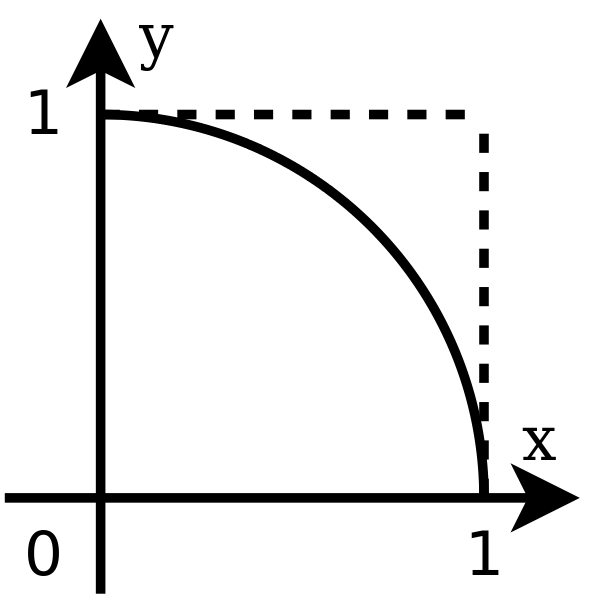
\includegraphics[width=0.9\textwidth]{pi.png}
\end{figure}
\end{column}
\end{columns}
\end{frame}

\begin{frame}
\frametitle{Case Study: Calculating $\pi$}
\begin{columns}
\begin{column}{0.6\textwidth}
\begin{itemize}
\small{
\item We can't calculate the area ratio without knowing $\pi$
\item Estimate it by:
\begin{itemize}
	\item Randomly picking many points inside the square
	\item Test if the point is inside the circle with $x^2 + y^2 < 1$
	\end{itemize}
}
\end{itemize}
\end{column}
\begin{column}{0.4\textwidth}
\begin{figure}
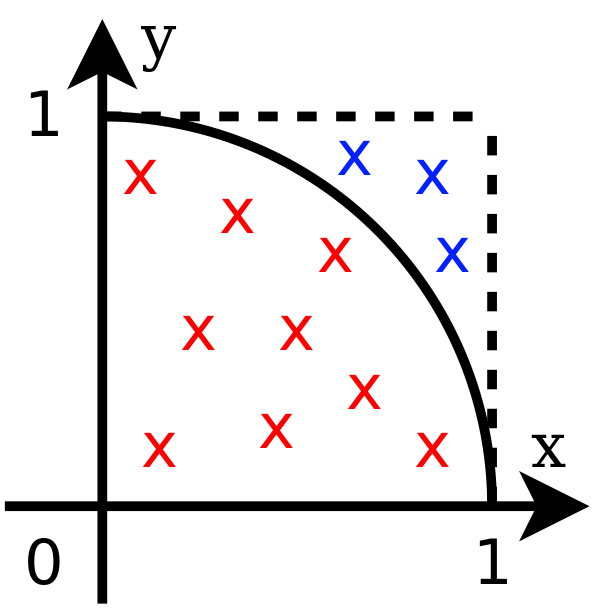
\includegraphics[width=0.9\textwidth]{pi-dots.png}
\end{figure}
\end{column}
\end{columns}
\begin{itemize}
\item $\pi \approx 4 \times \frac{\textrm{Number of points which land inside circle}}{\textrm{Total number of points tested}} = 4 \times \frac{9}{12} = 3$
\end{itemize}
\end{frame}

\begin{frame}
\frametitle{Algorithm for Calculating $\pi$}

\begin{itemize}
\item How can the above \textit{mathematics} be turned into an \textit{algorithm}?
	\begin{itemize}
		\item \textbf{NB:} You only have to understand the algorithm
	\end{itemize}
\pause
\item The algorithm needs to repeat the \textit{same thing} multiple times
	\begin{itemize}
			\item This implies use of a loop
			\item The loop's \textit{exit condition} needs to be defined
	\end{itemize}
\pause
\item As the loop repeats, we need to keep track of the following \textit{variables}:
		\begin{itemize}
			\item The number of points tested
			\item The number of points which landed inside the circle
			\item The $(x,y)$ coordinates of the point under test
		\end{itemize}


\end{itemize}	 
\end{frame}

\begin{frame}
\frametitle{Algorithm for Calculating $\pi$}
\begin{itemize}
\item The number of points tested will be an integer, we will call it \texttt{countTotal}
\item The number of points found to be inside the circle is also an integer, we will call it \texttt{countInside}
\item Before these variables are used they should be \textit{initialised}
	\begin{itemize}
		\item ie: The algorithm will explicitly include \texttt{countTotal = 0} and \texttt{countInside = 0}
		\item So-called \textit{uninitialised} variables have undefined (or random) values
	\end{itemize}
\end{itemize}
\end{frame}

\begin{frame}
\frametitle{Algorithm for Calculating $\pi$}
\begin{itemize}
\item Incrementing the \texttt{countInside} variable is \textit{conditional} on the values of $x$ and $y$
	\begin{itemize}
		\item This implies \texttt{IF...ENDIF} \textit{flow control}
	\end{itemize}
\pause
\item The condition on incrementing \texttt{countInside} is $x^2 + y^2 < 1$
\pause
\item Incrementing a variable in pseudocode takes the form:
	\begin{itemize}
		\item \texttt{variable = variable + 1}
		\item This can be read as ``variable \textit{becomes} variable plus 1''
		\item Maths people would write: $x_{n+1} = x_n + 1$
	\end{itemize}
\end{itemize}
\end{frame}

\begin{frame}
\begin{itemize}
\item The point under test needs two ``real'' variables: \texttt{x} and \texttt{y}
	\begin{itemize}
 		\item ``Real'' comes from mathematics: any number with integer and fractional components. Eg: 1.45
	\end{itemize}
\item These values take new random values each loop
\item The pseudocode doesn't need to describe how a random number is generated
	\begin{itemize}
		\item Stating: ``\texttt{x = a random number between 0 and 1}'' is totally acceptable
	\end{itemize}
\item At the end of the algorithm the final step will be $\pi = 4\times \frac{\texttt{countInside}}{\texttt{countTotal}}$
\end{itemize}
\end{frame}


\begin{frame}[fragile]
\frametitle{Algorithm for Calculating $\pi$}
\begin{lstlisting}[style=pseudo]
BEGIN
	integer countTotal = 0
	integer countInside = 0
	WHILE countTotal < A large number
		x = random number between 0 and 1
		y = random number between 0 and 1
		countTotal = countTotal + 1
		IF x*x + y*y < 1
			countInside = countInside + 1
		ENDIF
	ENDWHILE
	pi = 4*countInside/countTotal
	PRINT pi
END
\end{lstlisting}
\end{frame}

\begin{frame}
\frametitle{Missing Knowledge for C Implementation}
\begin{itemize}
\item More information about arithmetic
\begin{itemize}
	\item Relational operators (less/greater-than) look useful
	\item Is there a neat way to do \texttt{count=count+1}?
	\item \texttt{countInside} and \texttt{countTotal} are both integers. What happens when we divide?
\end{itemize}
\item Datatypes and how they are handled in arithmetic statements
\item How do we generate random numbers?
\item Syntax for WHILE loops and IF statements
\end{itemize}
\end{frame}

\begin{frame}
\frametitle{C Arithmetic}
\begin{itemize}
\item Basic arithmetic was seen in the lab
\begin{table}[H]
\centering
\begin{tabular}{|l|c|}
\hline
Operation      & C Symbol \\
\hline
Addition       & \texttt{+}        \\
Subtraction    & \texttt{-}        \\
Multiplication & \texttt{*}        \\
Division       & \texttt{/}       \\
\hline
\end{tabular}
\caption{Basic arithmetic operators in C}
\end{table}
\item Complex expressions can be built from these operators and parentheses
\end{itemize}
\end{frame}

\begin{frame}
\frametitle{C Arithmetic}
Examples:
\begin{small}
\begin{table}
\centering
\begin{tabular}{cc}
\vspace{2mm}
$z = x^2 + 5(y + b)$ & \texttt{z = x*x + 5*(y + b);} \\
\vspace{2mm}
$u = \frac{x + 1}{x - 1}$ & \texttt{u = (x + 1)/(x - 1);} \\
$v = z^3 + \frac{5(y + b)}{2}$ & \texttt{v = z*z*z+(5*(y + b))/2;} \\
\end{tabular}
\end{table}
\end{small}

\begin{itemize}
\item Multiplication is not assumed. If you write \texttt{5(y+b)} the compiler will generate a syntax error.
\item To be valid C statements the semicolon is required.
\end{itemize}
\end{frame}

\begin{frame}
\frametitle{C Arithmetic}
\begin{itemize}
\item C supports two time-saving \textit{unary} operators:
\begin{itemize}
\item Very useful in loops.
\end{itemize}

\begin{table}
\centering
\begin{tabular}{|c|c|c|}
\hline
Operation & C Syntax & Replaces\\
\hline
Increment & \texttt{x++;} or \texttt{++x;} & \texttt{x = x + 1;} \\
Decrement & \texttt{x--;} or \texttt{--x;} & \texttt{x = x - 1;} \\
\hline
\end{tabular}
\end{table}

\item It also supports the following shorthand syntax:

\begin{table}
\centering
\begin{tabular}{|c|c|c|}
\hline
\texttt{x = x + y;} & \texttt{x += y;} \\
\texttt{x = x - y;} & \texttt{x -= y;} \\
\texttt{x = x * y;} & \texttt{x *= y;} \\
\texttt{x = x / y;} & \texttt{x /= y;} \\
\hline
\end{tabular}
\end{table}
\end{itemize}
\end{frame}

\begin{frame}
\frametitle{C Arithmetic}
What's the difference between \texttt{x++} and \texttt{++x}?
\begin{itemize}
\item \texttt{x++} is a \textit{post-increment}
\item \texttt{++x} is a \textit{pre-increment}
\item If they appear in an arithmetic expression, pre-increment is processed \textit{before} the variable is used and post-increment is processed \textit{after} it is used.
\item In isolation there is no difference.
\end{itemize}
\end{frame}



\begin{frame}
\frametitle{Modulus}
\begin{itemize}
\item Integer division ignores (truncates) any fractional component
\item The \textit{modulus} operator provides the remainder after division
\begin{itemize}
	\item C uses the \texttt{\%} character
	\item ``\texttt{a \% b}'' means ``remainder of \texttt{a / b}''
\end{itemize}
\item Example:
	\begin{itemize}	
		\item \texttt{10 / 3 = 3}
		\item \texttt{10 \% 3 = 1}
	\end{itemize}
\end{itemize}
\end{frame}

\begin{frame}[fragile]
\frametitle{Modulus Example - Printing Every \textit{nth} Number}
\begin{lstlisting}[style=CStyle]
#include <stdio.h>
int main() {
	int x = 0;
	while(x < 1000)
	{
		x++; // Increment x
		if(x%100 == 0) // if(x is divisible by 100)
			printf("%d\n", x);
	}
	return 0;
}
\end{lstlisting}
\end{frame}

\begin{frame}
\frametitle{Relational Operators}
\begin{itemize}
\item C supports six \textit{relational} operators:
\begin{table}[H]
\centering
\begin{tabular}{|l|c|}
\hline
Operation      & C Symbol \\
\hline
Less than       & $\texttt{<}$        \\
Less than or equal to    & $\texttt{<=}$\\
Greater than & $\texttt{>}$        \\
Greater than or equal to       & $\texttt{>=}$       \\
Equal to & \texttt{==} \\
Not equal to & \texttt{!=} \\
\hline
\end{tabular}
\end{table}
\end{itemize}
\end{frame}

\begin{frame}
\frametitle{Relational Operators}
\begin{itemize}
\item The result of a relational operation is \texttt{0} or \texttt{1}
	\begin{itemize}
		\item C treats \texttt{0} as Boolean FALSE and non-zero as TRUE
	\end{itemize}
\item They are typically used as flow control conditions
	\begin{itemize}
		\item \texttt{if(\textit{condition}) \{\textit{statements}\}}
		\item \texttt{while(\textit{condition}) \{\textit{statements}\}}
	\end{itemize}
\item While we're here: the above is the correct syntax for IF and WHILE flow control in C
\end{itemize}
\end{frame}

\begin{frame}[fragile]
\frametitle{\texttt{if()} and \texttt{while()}}
\begin{itemize}
\item Syntax for your ``cheat sheet'':

\begin{lstlisting}[style=CStyle]
if(condition) {
	// Do stuff
}
\end{lstlisting}

\begin{lstlisting}[style=CStyle]
if(condition) {
	// Do stuff
} else {
	// Do other stuff
}
\end{lstlisting}

\begin{lstlisting}[style=CStyle]
while(condition) {
	// Do stuff
}
\end{lstlisting}
\item If there is a single \textit{statement} inside an \texttt{if()} or \texttt{while()} the \texttt{\{} and \texttt{\}} are optional
\end{itemize}
\end{frame}

\begin{frame}[fragile]
\frametitle{\texttt{if()} and \texttt{while()}}
Example:
\begin{lstlisting}[style=CStyle]
#include <stdio.h>

main() {
	while(x != 0) {
		scanf("Enter an integer: %d\n", &x);
		if(x % 2 == 0)
			printf("%d is even\n", x);
		else
			printf("%d is odd\n", x);
	}
}
\end{lstlisting}
\end{frame}


\begin{frame}
\frametitle{Boolean Operators}
\begin{itemize}
\item We discussed Boolean algebra last week
\item It has three operators: AND, OR, NOT
\item In C, these are implemented with:
\end{itemize}
\vspace{-5mm}
\begin{table}[]
\begin{tabular}{|c|c|}
\hline
Operator & C Characters \\
\hline
AND      & \texttt{\&\&}         \\
OR       & \texttt{||}           \\
NOT      & \texttt{!}           \\
\hline
\end{tabular}
\end{table}
\vspace{-5mm}
\begin{itemize}
\item I know the \texttt{|} character as a ``pipe'' symbol or ``vertical slash''
	\begin{itemize}
		\item Ask your demonstrator to find it on the keyboard
	\end{itemize}
\end{itemize}
\end{frame}

\begin{frame}
\frametitle{Conditions}
\begin{itemize}
\item We have seen that \texttt{if()} and \texttt{while()} statements need \textit{conditions}
\item A condition can be any combination of variables, operators, and literals (numbers, defined later)
\item The following are all valid:
	\begin{itemize}
		\item \texttt{if(x > 29)}
		\item \texttt{if(x == 2)}
		\item \texttt{if(!(x == y))}
		\item \texttt{if( (x > 5) \&\& (x < 20) )}
		\item \texttt{if(x = y + z)}
			\begin{itemize}
				\item Evaluates \texttt{(y + z)}, assigns to \texttt{x}, uses result as \texttt{if()} condition.
			\end{itemize}
	\end{itemize}
\end{itemize}
\end{frame}

\begin{frame}
\frametitle{C Arithmetic Operator Precedence}
\begin{itemize}
\item C has an ``order of operations''
\item eg: \texttt{1+5*2} evaluates to \texttt{11}
	\begin{itemize}
		\item You remember BODMAS / PEDMAS, right?
	\end{itemize}
\item Multiplication and division first
\item Addition and subtraction second
\item Relational operators somewhere below that
\item If in doubt: force order with parentheses
	\begin{itemize}
		\item This makes the code more readable
		\item It doesn't cost you anything
		\item C compilers understand algebra and will optimise inefficient expressions automatically
	\end{itemize}

\end{itemize}
\end{frame}

\begin{frame}
\frametitle{Variable Declaration}
\begin{itemize}
\item In C, all variables are \textit{declared} before use
\item Declaration specifies the variable's:
	\begin{itemize}
		\item Datatype
		\item Name
		\item An \textit{initialisation value} (optional)
			\begin{itemize}
				\item Always assume uninitialised variables have random values! Behaviour varies between compilers and target platforms.
			\end{itemize}
		\item eg: \texttt{int counter = 0;}
			\begin{itemize}
				\item Type is \texttt{int}
				\item Name is \texttt{counter}
				\item Initial value is \texttt{0} (optional)
			\end{itemize}
	\end{itemize}
\item C is a ``strongly-typed'' language
	\begin{itemize}
		\item A variable's type doesn't change
	\end{itemize}
\end{itemize}
\end{frame}

\begin{frame}[fragile]
\frametitle{Variable Declaration}
\begin{itemize}
\item You can declare multiple variables in one line:
\begin{lstlisting}[style=CStyle]
int a, b, c, d;
\end{lstlisting}
\item You can mix initialised and uninitialised variables:
\begin{lstlisting}[style=CStyle]
float q, r = 1.0, s = 12e3, t;
\end{lstlisting}
\item All variables declared in this way must be of the same type
\end{itemize}
\end{frame}

\begin{frame}
\frametitle{Variable Naming Rules}
\begin{itemize}
\item Variable names:
	\begin{itemize}
		\item Are case sensitive
		\item Must \textbf{not} be a C keywoard (eg: \texttt{int, char, while}, etc)
		\item Must \textbf{not} contain special characters (\texttt{*-+/,} etc)
		\item Must begin with a letter
		\item Can contain numbers
		\item Can contain underscores
		
	\end{itemize}
\item What you do with those rules is up to you
\item Modern practice encourages:
	\begin{itemize}
		\item camelCaseVariableNames
		\item names\_with\_underscores
	\end{itemize}
\end{itemize}
\end{frame}

\begin{frame}
\frametitle{Integer Data Types}
\begin{itemize}
\item There are several integer data types
\item They vary by their:
	\begin{itemize}
		\item Size
		\item Support for negative numbers
	\end{itemize}
\item C integer types can be 1, 2, 4, or 8 bytes long
	\begin{itemize}
		\item \texttt{int} and \texttt{long} sizes vary by platform
		\item Larger sizes store larger numbers, use more RAM
	\end{itemize}
\item Each type can be \textit{signed} or \textit{unsigned}
	\begin{itemize}
		\item Unsigned numbers are always positive but you get double the \textit{value range}
	\end{itemize}
\end{itemize}
\end{frame}

\begin{frame}
\frametitle{Integer Data Types}
\begin{itemize}
\item The integer data type ranges can be calculated from the data type's size in bits
\item For unsigned numbers of bit length $n$:
\begin{equation}
\textrm{max} = 2^{n} - 1
\end{equation}
\item For signed numbers of bit length $n$:
\begin{align}
\textrm{max} &= 2^{(n-1)} - 1 \\
\textrm{min} &= -2^{(n-1)}
\end{align}
\item Signed numbers are stored in \textit{two's complement} format, covered in ELEC1710
\end{itemize}
\end{frame}

\begin{frame}
\frametitle{Integer Data Types}
\begin{itemize}
\item C includes the \texttt{sizeof()} expression so that a program can discover the size of a data type on a given platform
\item On a modern 64-bit Linux desktop machine:
\end{itemize}
\begin{table}[]
\begin{tabular}{llll}
Type & Bytes & Bits & Value Range                               \\
\texttt{char}      & 1            & 8           & -128, +127                                \\
\texttt{short}     & 2            & 16          & -32768, 32767      \\
\texttt{int}       & 4            & 32          & -2147483648, 2147483647                   \\
\texttt{long}      & 8            & 64          & -9223372036854775808, ...
\end{tabular}
\end{table}
\end{frame}

\begin{frame}
\frametitle{Unsigned Integers}
\begin{itemize}
\item Unsigned integers are \textit{always positive}
\item They are the same size as their signed counterparts
\item The \texttt{unsigned} keyword placed before the data type makes that variable unsigned
\item eg: \texttt{unsigned char} is 1 byte and has a value range of \texttt{0} to \texttt{255}
\end{itemize}
\end{frame}

\begin{frame}[fragile]
\frametitle{Overflow}
\small{
\begin{itemize}
\item \textit{Overflow} occurs when the result of a calculation is too big to fit into the target type
\item Example: \texttt{127 + 1 = -128}
\begin{lstlisting}[style=CStyle]
#include <stdio.h>
int main() {
	char x = 127;
	printf("%d\n", x);
	x++;
	printf("%d\n", x);
	return 0;
}
\end{lstlisting}

\end{itemize}
}
\end{frame}

\begin{frame}
\frametitle{Overflow}
\begin{itemize}
\item Message: make variables as small you can, but no smaller
	\begin{itemize}
		\item Or just use \texttt{long} everywhere and cop the performance hit
	\end{itemize}
\item Quite often you need to take a guess at how big a variable needs to be
\item Typically a good idea to document software limits due to variable choice
\end{itemize}
\end{frame}

\begin{frame}
\frametitle{Why Care About Data Types?}
\begin{itemize}
\item You may be thinking ``why not make everything a \texttt{long}?''
\item Answer: speed and memory
\item Smaller types use less RAM
\item Arithmetic on a type larger than the target platform's \textit{native size} is slow
\item Matters if you store millions of the same type
\item Makes a \textit{huge} difference on embedded targets
\begin{itemize}
	\item Don't declare 32-bit variables on an 8-bit AVR microcontroller \textit{unless you have to}
\end{itemize}
\end{itemize}
\end{frame}



\begin{frame}[fragile]
\frametitle{Floating Point Data Types}
\begin{itemize}
\item To store real numbers C has several \textit{floating point} data types
\item As with integers, try to use the smallest you can get away with
\item \texttt{long double} is supported in gcc but...\underline{\href{https://en.wikipedia.org/wiki/Long_double}{complicated}}
\end{itemize}

\begin{table}[] \small
\begin{tabular}{llll}
Type        & Size & Range                                             & Precision \\
float       & 4    & $1.2\times 10^{-38}$ to $3.4 \times 10^{38}$      & 6 dp      \\
double      & 8    & $2.3 \times 10^{-308}$ to $1.7 \times 10^{308}$     & 15 dp     \\   
\end{tabular}
\end{table}
\end{frame}

\begin{frame}
\frametitle{How good is 15 decimal places?}
Paraphrasing \underline{\href{https://www.jpl.nasa.gov/edu/news/2016/3/16/how-many-decimals-of-pi-do-we-really-need/}{NASA}}: \\
\vspace{5mm}
Calculating the circumference of Earth using 15 decimal places for $\pi$ results in a truncation error about the size of a molecule.\\
\vspace{5mm}
39 digits of $\pi$ calculates the circumference of the \textit{visible universe} to within the width of a hydrogen atom ($\approx10^{-10}$~m).

\end{frame}

\begin{frame}[fragile]
\frametitle{Floating Point Problems}
\begin{itemize}
\item Q: Why not \textit{always} use \texttt{float} or \texttt{double} instead of \texttt{int}?
\item A: Floating point arithmetic is \textbf{\textit{NOT}} exact
\item Example 1: Does this code exit?
\begin{lstlisting}[style=CStyle]
#include <stdio.h>
int main() {
	float x = 16000000.0;
	while(x < 17000000.0) {
		x = x + 1.0;
		printf("%f\n", x);
	}
}
\end{lstlisting}
\end{itemize}
\end{frame}

\begin{frame}[fragile]
\frametitle{Floating Point Problems}
\begin{itemize}
\item Example 2: $\tan \left( \frac{\pi}{2} \right)$ is undefined
\item But using floating point $\pi$ can't be represented exactly, so C produces a result anyway
\begin{lstlisting}[style=CStyle]
#include <stdio.h>
#include <math.h>
int main() {
	double pi = 3.141592653589793238;
	printf("%f\n", tan(pi/2.0));
	printf("%f\n", ftanf((float)pi/2.0));
}
\end{lstlisting}
\end{itemize}
\end{frame}

\begin{frame}
\frametitle{Literals}
\begin{itemize}
\item A \textit{literal} is any number written in the code
\item Why not ``constant''?
	\begin{itemize}
		\item That word means something different
	\end{itemize}
\item Examples:
	\begin{itemize}
		\footnotesize{
		\item \texttt{x = 5; // 5 is a literal int}
		\item \texttt{y = 2.0 / z; // 2.0 is a literal double}
		}
	\end{itemize}
\item By default:
	\begin{itemize}
		\item An integer literal is stored  as an \texttt{int} data type
			\begin{itemize}
			 \item ie: has the value range and arithmetic limits of \texttt{int}
			\end{itemize}
		\item A floating point literal is stored as \texttt{double}
	\end{itemize}
\end{itemize}
\end{frame}

\begin{frame}
\frametitle{Literals}
\begin{itemize}
\item Integer literals can be in:
	\begin{itemize}
		\item Decimal: \texttt{123}
		\item Hexadecimal: \texttt{0xA34 // Zero-x}
		\item Octal: \texttt{O125 // Capital letter O}
		\item (Hex and octal are covered in ELEC1710)
	\end{itemize}
\item Integer literals can be specified as \textit{unsigned} with the \texttt{u} suffix:
	\begin{itemize}
		\item \texttt{938u}
	\end{itemize}
\item They can also be declared \texttt{long} with the \texttt{l} suffix:
	\begin{itemize}
		\item \texttt{3726484l}
		\item The compiler will issue a warning if a literal is too big for \texttt{int}
	\end{itemize}
\end{itemize}
\end{frame}

\begin{frame}
\frametitle{Literals}
\begin{itemize}
\item Floating point literals can be written in many ways:
	\begin{itemize}
		\item \texttt{1.0f // f suffix forces float}
		\item \texttt{(float)2.3 // Forces float}
		\item \texttt{1.0 // Default to double}
		\item \texttt{1e2 // Double, 1 times 10\^{}2}
	\end{itemize}
\item \texttt{1e2} is known as ``e-notation''
	\begin{itemize}
		\item \texttt{XeY} = $\texttt{X} \times 10^\texttt{Y}$
		\item I will use it \textit{all the time}
	\end{itemize}
\item Forcing literals to \texttt{float} is frequently necessary in embedded systems which lack double precision hardware
\end{itemize}
\end{frame}

\begin{frame}
\frametitle{Mixing Data Types}
\begin{itemize}
\item C supports arithmetic between different types
\item Type conversion is called \textit{casting}
\item When types are mixed two things can happen:
	\begin{itemize}
		\item Types get upgraded automatically (\textit{implicit} type casting)
			\begin{itemize}
				\item Upgrade path is roughly: \texttt{short/char - int - long - long long - float - double}
			\end{itemize}
		\item Types get specified manually by the programmer (\textit{explicit} type casting)
	\end{itemize}
\end{itemize}
\end{frame}

\begin{frame}
\frametitle{Explicit Type Casting}
\begin{itemize}
\item The data type of a variable (or literal) can be forced to change using \textit{type casting}
\item Write the desired type in parentheses before the variable or constant
\item Examples:
	\begin{itemize}
		\item \texttt{x = (float)y / k;}
		\item \texttt{y = (unsigned int)y + 32;}
	\end{itemize}
\end{itemize}
\end{frame}

\begin{frame}
\frametitle{Format Specifiers}
\begin{itemize}
\item A \textit{format specifier} controls how \texttt{printf();} converts numerical (or textual) data to a series of ASCII characters
\item Full details are complex, for now just use:
	\begin{itemize}
		\item \texttt{\%d} for integer types
		\item \texttt{\%f} for ``fixed decimal place'' floating point
		\item \texttt{\%e} for e-notation floating point
		\item Cast inside \texttt{printf()} to suppress compiler warnings
	\end{itemize}	 
\end{itemize}
\end{frame}

\begin{frame}[fragile]
\frametitle{Format Specifiers}
\begin{itemize}
\item Casting example:
\begin{lstlisting}[style=CStyle]
long i;
// ...
printf("%d\n", (int)i); //Breaks when i>2^31
\end{lstlisting}
\item \texttt{\%.df} produces \texttt{d} decimal places of precision
	\begin{itemize}
		\item eg: \\
		\begin{lstlisting}[style=CStyle]
float x = 1.23456;
printf("%.2f", x); // Prints 1.23
\end{lstlisting}
	\end{itemize}

\item Format specifiers can appear anywhere in the output text, eg:
\begin{lstlisting}[style=CStyle]
printf("%f was the result\n", x);
printf("The result %f was calculated\n", x);
\end{lstlisting}
\end{itemize}
\end{frame}

\begin{frame}[fragile]
\frametitle{Format Specifiers}
\begin{itemize}
\item You can print several numbers at once
\item Separate variables with commas
\item They are printed in the same order as variables are written
\item You can put maths inside \texttt{printf();}
\begin{lstlisting}[style=CStyle]
printf("%f plus %f is %f\n", x, y, x+y);
\end{lstlisting}
\end{itemize}
\end{frame}

\begin{frame}[fragile]
\frametitle{Integer Division Example}
With \textit{all that} out of the way, what is the output of each \texttt{printf()} statement?
\begin{lstlisting}[style=CStyle,caption=\texttt{intdiv.c}]
#include <stdio.h>
int main() {
	printf("%d\n", 9/10);
	printf("%f\n", 9/10);
	printf("%f\n", 9.0/10);
	printf("%f\n", 9/10.0);
	printf("%f\n", (float)9/10);
	return 0;
}
\end{lstlisting}
\end{frame}

\begin{frame}[fragile]
\frametitle{Random Numbers}
\begin{itemize}
\item In C there is a \textit{standard library function} which generates random numbers
\item We will study functions in more detail later
\item To use a library function:
	\begin{itemize}
		\item Read the function's documentation
		\item \texttt{\#include} the correct \textit{header file}
		\item Take note of the \textit{return value} data type
		\item Add any \textit{compiler flags} (beyond ENGG1003)
		\item Use the function in your code
	\end{itemize}
\item Demonstration: read the \texttt{rand()} man page
	\begin{itemize}
		\item Click \underline{\href{http://man7.org/linux/man-pages/man3/rand.3.html}{here}}
	\end{itemize}
\end{itemize}
\end{frame}

\begin{frame}[fragile]
\frametitle{Random Numbers}
\begin{itemize}
\item Observe that \texttt{rand();} requires 
\begin{lstlisting}[style=CStyle]
#include <stdlib.h>
\end{lstlisting}
\item Observe that it returns an \texttt{int} between 0 and \texttt{RAND\_MAX} which, in gcc, is $2^{31}-1$
\item Note that is has \underline{\href{http://www.azillionmonkeys.com/qed/random.html}{limits}} (advanced discussion, beyond ENGG1003)
\item For us, using the \% operator:
\begin{lstlisting}[style=CStyle]
x = rand() % (RANGE+1);
\end{lstlisting}
produces a \textit{good enough} random number between zero and \texttt{RANGE}
\end{itemize}
\end{frame}

\begin{frame}[fragile]
\frametitle{Random Numbers}
\begin{itemize}
\item As above, zero to \texttt{RANGE} is produced with:
\begin{lstlisting}[style=CStyle]
x = rand() % (RANGE+1);
\end{lstlisting}
\item To generate numbers from 1 to \texttt{RANGE}:
\begin{lstlisting}[style=CStyle]
x = (rand() % RANGE) + 1;
\end{lstlisting}
\item These work because:
\begin{lstlisting}[style=CStyle]
x = rand() % MAX;
\end{lstlisting}
is a random number between zero and \texttt{(MAX-1)}
\end{itemize}
\end{frame}

\begin{frame}[fragile]
\frametitle{Random Numbers}
\begin{itemize}
\item Using the above information, we can roll a standard die with:
\begin{lstlisting}[style=CStyle]
int dieRoll;
dieRoll = (rand() % 6) + 1;
\end{lstlisting}
\item Or, if you're a D\&D fan, roll a D20 with:
\begin{lstlisting}[style=CStyle]
int D20Roll;
D20Roll = (rand() % 20) + 1;
\end{lstlisting}
\end{itemize}
\end{frame}


\begin{frame}[fragile]
\frametitle{Random Numbers}
\begin{itemize}
\item \texttt{RAND\_MAX} is a \textit{constant} defined in \texttt{stdlib.h}
\item We can try to generate a floating point number from 0 to 1 with a division:
\begin{lstlisting}[style=CStyle]
float num;
num = rand()/RAND_MAX; // This is broken
\end{lstlisting}
\item Problem: \texttt{rand()} is an integer, \texttt{RAND\_MAX} is a (large) integer
	\begin{itemize}
		\item The integer division result will always be zero!
	\end{itemize}
\item Solution: use an explicit cast so that a floating point division occurs:
\begin{lstlisting}[style=CStyle]
double num;
num = (double)rand()/RAND_MAX;
\end{lstlisting}
\end{itemize}
\end{frame}

\begin{frame}
Probably out of time by now, lets implement a $\pi$ calculator in the lab... \textit{In theory} you have enough information by now.
\end{frame}

\end{document}
